\chapter{Introduction}

\section{Motivation}
One of the keys factors that has driven transformation of computing industry in the last years is the perception of computing utilities as an ordinary property\cite{BuYeVeBrBr09}, which can be easily accessed and adjusted to a specific needs. That point of view resulted in profusion of different services, often collectively referred as a cloud computing \cite{MeGr11}. Similarly to services common to traditional markets, customers expect them to be accessible on demand and in easy manner, while paying only for the consumed goods. Furthermore, customers are interested in a given service provider only when it is eligible to guarantee appropriate quality of service.

The particular service providers that are addressed by this paper are the ones that supply users with an application execution platform, what is widely known as providing Platform-as-a-Service. In that case, a customer is an entity that has developed application and is eager to deploy it on an application platform that is able to fulfil his specific requirements, both in terms of quality and cost.

Having customer requirements in mind, it is crucial that service provider is able to adapt itself to meet them. For example, such adaptation can be triggered by a sudden spike in resource demand and may result in provisioning additional application platforms. However, due to the complexity of a system under consideration, there are different levels where adaptation is possible:
\begin{itemize}
	\item user application
	\item application platform
	\item infrastructure
\end{itemize} 
What is more, the fact that single service provider is constrained by his finite amount of resources poses a risk that it may not be able to serve customer all the time. Consequently, it is expected that adaptation at a service provider level is also possible, i.e. provider can offload some traffic to a different provider, as long as it satisfies a customer.

While autonomic computing has a long history \cite{Mu04}, it has not been directly applied to a multi-layered problem that exists in a cloud computing environment. Especially, the research area at the last layer, which sizes across different service providers, is new. Although, architecture known as InterCloud \cite{BuRaCa10} investigates problem of cooperation and negotiation at cloud level, it neither has been implemented nor presented in context of autonomic system.

\subsection{Business potential}
The rapid growth of interest in cloud computing in recent years resulted in huge sums of money being invested in the field. Figure \ref{chapter-fig:public-cloud-services-market-size} shows the size of the public cloud services market in 2012 and the forecast of its nearly two times growth in 2016. This data suggests that the subject is attractive for IT industry from the economic point of view. However, higher amounts of money spent on cloud services involve higher expectations of theirs quality from customers. Although the most significant players in cloud computing have been in the field for quite a long time, it is still possible to outline some deficiencies their products have. Additionally, lack of common standards hinder cooperation among different cloud providers. For example it is nearly impossible to create an autoscaling cloud federation with Amazon Web Services (current leader in providing cloud services\cite{GartnerMagicQuadrantSep2013}) and another provider. What is more, Amazon AWS users cannot use more lightweight virtualization methods, such as linux containers. Nevertheless, when compared to other companies especially in terms of autoscaling capabilities, Amazon really shines. OpenShift, RedHat PaaS solution, ensures application scaling but with very limited possibilities of customisation of the process -- the user can only choose if their application should scale and the whole algorithm is solely based on the number of concurrent requests to the application. Users of Heroku, another PaaS solution, have no automation tool that would control the number of instances (\emph{dynos} in Heroku nomenclature) their application is running on -- they can change it manually.

The proposed solution in this dissertation tries to deal with the aforementioned providers problems by outlining an example architecture that enables seamless cooperation among cloud providers and provides auto-scaling capabilities.

\begin{figure}[!ht]
  \begin{center}
    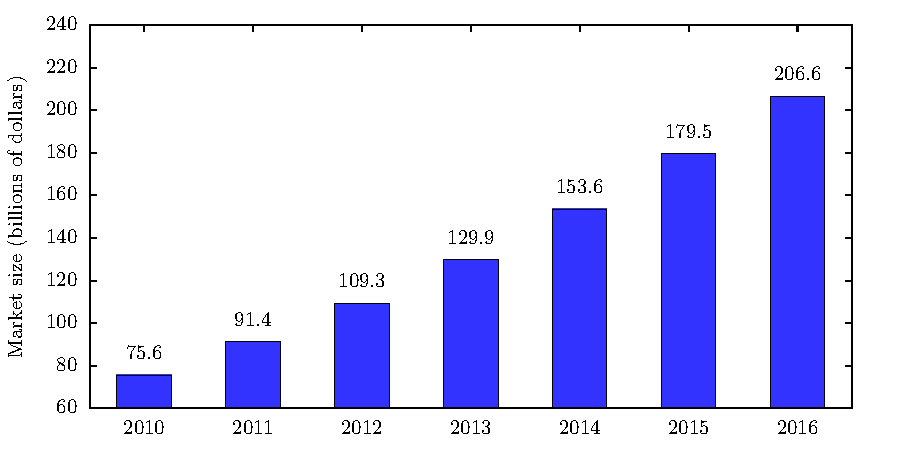
\includegraphics{chapter-introduction/public-cloud-services-market-size}
  \end{center}
  \caption{Public Cloud Services Market Size, 2010-2016 (forecast). Source: \textit{Gartner, 08/2012}}
  \label{chapter-fig:public-cloud-services-market-size}
\end{figure}

\section{Contributions}
The main contributions of this dissertation are as follows:
\begin{itemize}
  \item A proposal of an architecture of federated cloud computing environment, which is based on and can be viewed as a simplified version of \emph{InterCloud}
  \item The notion of considering each service model as an autonomic system
  \item The implementation of the proposed architecture using OpenNebula technology stack
\end{itemize}

\section{Impact}
We hope that the concept of representing each level of an autoscaling subsystem as an autonomic one can be thought-provoking for cloud computing scientists.  What is more, we believe that our successful attempt to implement a simplified variant of an InterCloud architecture will cause its gain in interest and popularity. 
Finally, we consider the ideas contained in this work be beneficial to the OpenNebula ecosystem as they provide insights into the ways Quality of Service can be ensured:
\begin{itemize}
  \item implementing autoscaling capabilities
  \item designing \emph{cloud infrastructure} in accordance with InterCloud architecture
\end{itemize}

\section{Thesis structure}
